\section{Setting the target domain} \label{sec:domain}
%=======================================================================

This section explains the number of grids, and the target domain and its relationship with the MPI process. The calculation domain is determined by the horizontal grid spacing, the number of grid points, and the number of MPI processes. Figure \ref{fig:domain} gives an example of this relationship. The parallelization is implemented by a 2D domain decomposition in the horizontal direction.

The numbers of grids and of MPI processes are specified in \nmitem{IMAX, JMAX} in \namelist{PARAM_INDEX}, and in \nmitem{PRC_NUM_X, PRC_NUM_Y} in \namelist{PARAM_PRC}, respectively. As shown in Fig. \ref{fig:domain},  the entire domain is divided into \nmitem{PRC_NUM_X} along the X direction and \nmitem{PRC_NUM_Y} in the Y direction. Each sub-domain is managed by an MPI process, each of which takes charge of a grid block of IMAX $\times$ JMAX $\times$ KMAX. Care is taken to ensure that this number of grids is taken charge of by one process: its value is not identical to the total number of grids in the domain. In other words, the entire domain depends on the number of MPI processes, the horizontal grid spacing, and the number of grids.

Thus, the number of grids along each horizontal direction and that in the entire domain are derived as follows:
\begin{eqnarray}
&& \verb|Number of grids in the X direction| = \verb|IMAX| \times \verb|PRC_NUM_X|
   \label{eq:xgridnum}\\
&& \verb|Number of grids in the Y direction| = \verb|JMAX| \times \verb|PRC_NUM_Y|
   \label{eq:ygridnum}\\
&& \verb|Total number of grids in the domain| \nonumber\\
&& = \left(\verb|IMAX| \times \verb|PRC_NUM_X|\right)
   \times (\verb|JMAX| \times \verb|PRC_NUM_Y|)
   \times (\verb|KMAX| ),
\end{eqnarray}
where \nmitem{KMAX} is the number of grids along the vertical direction, which is specified in \namelist{PARAM_INDEX}.

By using Eqs. (\ref{eq:xgridnum} and \ref{eq:ygridnum}),  the size of the entire domain is determined as follows:
\begin{eqnarray}
&& \verb|Domain length in the X direction| = \verb|number of grids in the X direction| \times \verb|DX|\\
&& \verb|Domain length in the Y direction| = \verb|number of grids in the Y direction| \times \verb|DY|,
\end{eqnarray}
where \nmitem{DX, DY} is grid spacings specified  in \namelist{PRAM_GRID} as described in subsection \ref{subsec:gridinterv}.
If the horizontal resolution and domain size are set and the available number of MPI processes is given, the number of grids that are controlled by one MPI process can be determined as in the above relationship.

In the next subsections, the configuration of the MPI processes, the number of grids, and the grid interval are described in more detail.  \textcolor{blue}{Note that it is necessary that these settings  be identical among the configuration files \texttt{pp.conf},  \texttt{init.conf}, and \texttt{run.conf}}.

\begin{figure}[h]
\begin{center}
  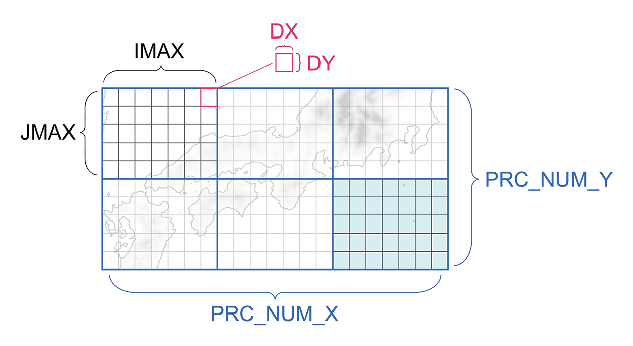
\includegraphics[width=0.8\hsize]{./figure/domain_decomposition.eps}\\
  \caption{Relation between horizontal grid interval (\texttt{DX}, \texttt{DY}), number of grids (\texttt{IMAX}, \texttt{JMAX})
    per MPI process, and the number of MPI processes (\texttt{PRC\_NUM\_X}, \texttt{PRC\_NUM\_Y})     in the entire domain. The light-blue part corresponds to a region managed by an MPI process.}
  \label{fig:domain}
\end{center}
\end{figure}

%-----------------------------------------------------------------------
\subsection{Setting the number of MPI processes} \label{subsec:relation_dom_reso2}
%-----------------------------------------------------------------------

The number of MPI processes is specified in \namelist{PARAM_PRC} in the configuration file. Since the input and output files of \scalerm are divided process by process according to the MPI, the total number of files is changed according to the number of MPI processes. For example, the initial condition file made by a two-MPI parallel combination cannot be used for model execution by a four-MPI parallel.
It is necessary to edit \namelist{PARAM_PRC} in \verb|pp.conf|, \verb|init.conf|, and \verb|run.conf| if the number of MPI processes is changed,
and to conduct once again the processes of \verb|pp| and \verb|init|.
\editboxtwo{
\verb|&PARAM_PRC| & \\
\verb| PRC_NUM_X       = 2,| & ; number of divisions by MPI parallelization in the {\XDIR}(zonal direction)\\
\verb| PRC_NUM_Y       = 1,| & ; number of divisions by MPI parallelization in the {\YDIR}(meridional direction)\\
\verb|/|\\
}
The total number of MPI processes is given by \verb|PRC_NUM_X| $\times$ \verb|PRC_NUM_Y|.
The above example expresses a two-MPI parallel by dividing the domain into two sub-domains along the X direction, but not dividing along the Y direction. The total number of processes must be given as the number of MPI processes in the MPI command at submitting job. If this condition is not satisfied,  the program is terminated immediately without calculation and the following message is output to the standard output.
\msgbox{
\verb|xxx total number of node does not match that requested. Check!| \\
}

%-----------------------------------------------------------------------
\subsection{Setting the number of horizontal and vertical grids} \label{subsec:relation_dom_reso3}
%-----------------------------------------------------------------------

The number of grids is specified in \namelist{PARAM_INDEX} in the configuration files \verb|***.conf|. It should be noted that the specified horizontal grids are values controlled by one MPI process.
\editboxtwo{
\verb|&PARAM_INDEX| & \\
\verb| KMAX = 97,|  & ; number of vertical layers \\
\verb| IMAX = 20,|  & ; number of grids along the X direction by an MPI process\\
\verb| JMAX = 25,|  & ; number of grids along the Y direction by an MPI process\\
\verb|/|\\
}

%-----------------------------------------------------------------------
\subsection{Setting grid intervals along the horizontal and vertical directions} \label{subsec:gridinterv}
%-----------------------------------------------------------------------

Excluding the buffer region explained in Section \ref{subsec:buffer}, the horizontal grid intervals are configured only equidistantly, whereas the
 vertical grid intervals are configured freely. When the grid intervals are  configured uniformly along all directions, specify the zonal, meridional, and vertical grid intervals  at \nmitem{DX, DY, DZ} in \namelist{PARAM_GRID}, respectively. The unit is [m].
\editboxtwo{
\verb|&PARAM_GRID  | & \\
\verb| DX = 500.D0,| & ; grid interval along the zonal (X) direction\\
\verb| DY = 500.D0,| & ; grid interval along the meridional(Y)direction\\
\verb| DZ = 500.D0,| & ; grid interval along the vertical (Z) direction\\
\verb|/|\\
}

The box below shows the method to set how to specify a non-uniform grid system.
Since the model employs the Lorenz grid system, the points of definition for the velocity vector and other scalars are staggered, deviating by a half grid.
In this document, the scalar location is called the center point and the half-grid-deviated location the face point.
When the vertical grid locations are directly specified, provide them in \nmitem{FZ(:)} in \namelist{PARAM_GRID} as an array.\footnote{In this case, the same precision as used in the simulation is recommended to be specified. By default, the model is compiled as a double-precision floating point model.} Refer to Figure \ref{fig:scale_grid} for the details. Note that the number of elements specified in \nmitem{FZ(:)} should correspond to the number of vertical layers (\nmitem{KMAX} in \namelist{PARAM_INDEX}). The following file for the ideal experiment is shown as an example:
\editboxtwo{
\verb|&PARAM_GRID|     & \\
\verb| DX = 500.D0,|   & grid interval along the X direction (equidistant) [m]\\
\verb| DY = 500.D0,|   & grid interval along the Y direction (equidistant) [m]\\
\verb| FZ(:) = |       & location at face point along the Z direction [m] \\
\verb|    80.000000000000000      ,| & \\
\verb|    168.00000190734863      ,| & \\
\verb|    264.80000610351567      ,| & \\
\verb|     ........ |           & \\
\verb|    14910.428862936289      ,| & \\
\verb|    15517.262523292475      ,| & \\
\verb|    16215.121232702089      ,| & \\
\verb|    17017.658748523147      ,| & \\
\verb|    17940.576891717363      ,| & \\
\verb|    19001.932756390710      ,| & \\
\verb|    20222.492000765058      ,| & \\
\verb| BUFFER_DZ = 5000.D0,|          & Refer to Section \ref{subsec:buffer}\\
\verb| BUFFFACT  =   1.0D0,|          & Refer to Section \ref{subsec:buffer}\\
\verb|/|\\
}

\begin{figure}[tb]
\begin{center}
  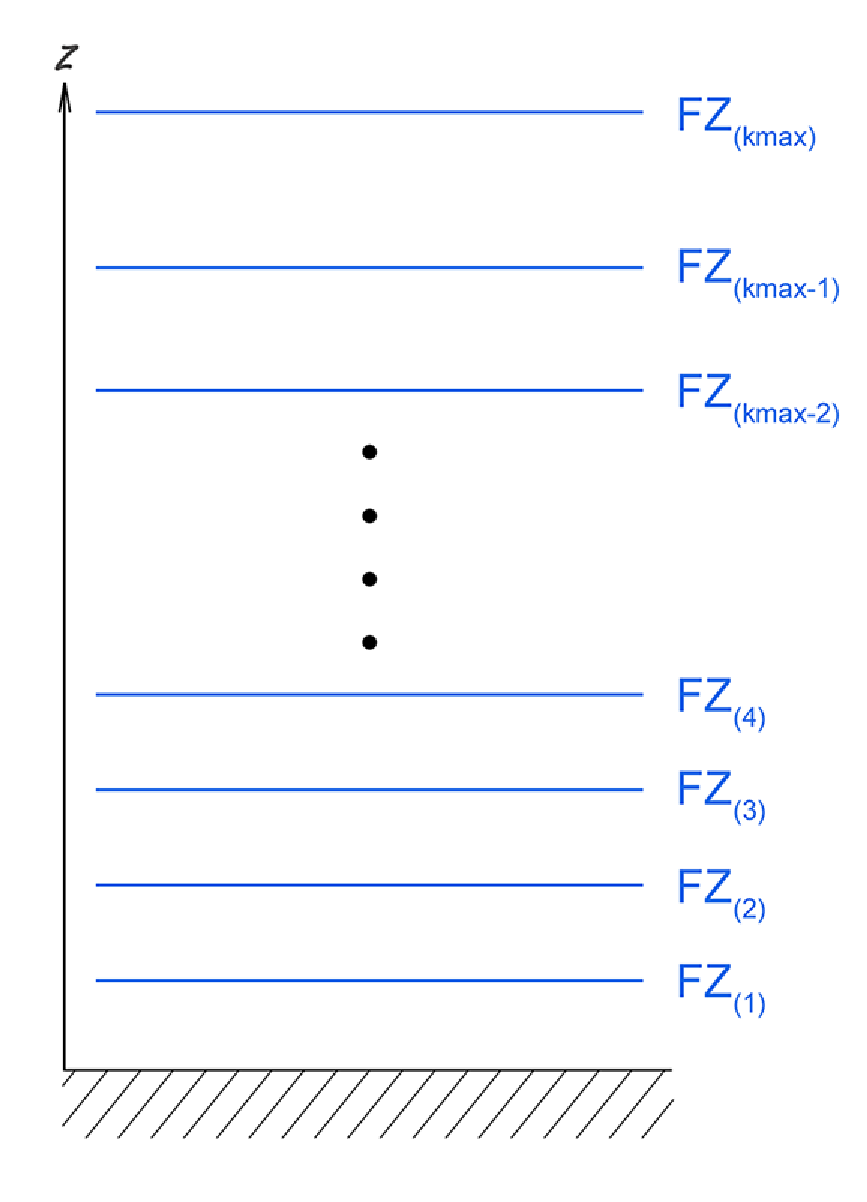
\includegraphics[width=0.4\hsize]{./figure/verticalface.eps}\\
  \caption{The point of definition of the face point in \scalerm. If \nmitem{FZ} is given in \namelist{PARAM_GRID}, the top height at the first layer is given for the value at $k=1$. Note that $k=1$ is not the ground surface height.}
  \label{fig:scale_grid}
\end{center}
\end{figure}

The above setting is processed at a topographical height of 0 m.
The location of the vertical grids at the non-zero topography is appropriately treated by the terrain-following coordinate.

The locations of the vertical grids are configured freely.
However, an unusual configuration sometimes leads to numerical instability. To avoid it, the tool for the generation of vertical grids is supported as a FORTRAN program \verb|make_vgrid.f90| in the directory\\ \texttt{scale-\version/scale-rm/util/makevgrid/} with several samples of the namelist. If needed, use them as references. The tool generates the values of \nmitem{FZ(:)} directly. Copy and paste them in the configuration file.

%-----------------------------------------------------------------------
\subsection{Setting sponge layer} \label{subsec:raydamp}
%-----------------------------------------------------------------------

\scalerm adopts height coordinate system in vertical. The uppermost boundary condition is a rigid lid, and the sound and gravity waves often reflect at the model top. To reduce worse effects of these reflecting waves, the damping layer named ``sponge layer'' is placed in the upper part of the model domain. In the sponge layer, a vertical velocity is dumped by Rayleigh friction. The relaxation time scale (= e-folding time) of damping is minimum at the model top and it increases with decreasing the height. Below the bottom boundary of sponge layer, the relaxation time scale is set to infinity.
There are two methods to set the thickness of the sponge layer in \namelist{PARAM_ATMOS_DYN}.

\begin{enumerate}
\item specify number of layer of the sponge layer \\
  The number of layer appointed in \nmitem{ATMOS_DYN_wdamp_layer} is set as the sponge layer. The number is counted from the model top.
\item specify bottom boundary height [m] of the sponge layer \\
  The layer that is higher than altitude appointed in \nmitem{ATMOS_DYN_wdamp_height} is set as the sponge layer.
\end{enumerate}

Both parameters above are not set by default, and the sponge layer is not applied. If both are set, \nmitem{ATMOS_DYN_wdamp_layer} is given priority.

The relaxation time at the uppermost boundary is specified by \nmitem{ATMOS_DYN_wdamp_tau}. The unit is [second]. This parameter is not allowed to set the value smaller than \nmitem{TIME_DT_ATMOS_DYN}. When \nmitem{ATMOS_DYN_wdamp_tau} is not specified explicitly, the value ten times as large as \\
\nmitem{TIME_DT_ATMOS_DYN} is automatically set. Please refer to section \ref{sec:timeintiv} for \nmitem{TIME_DT_ATMOS_DYN}.
The example of concrete setting is shown in section \ref{subsec:atmos_dyn_scheme}.

%-----------------------------------------------------------------------
\subsection{Setting the buffer region and boundary nudging method} \label{subsec:buffer}
%-----------------------------------------------------------------------

In general, disagreement in values between input data as boundary condition and actual calculation output occurs at the lateral boundaries. They generate several problems, such as nonphysical mode, in calculation.
To avoid these problems, the ``buffer region'' is placed in the domain.

As shown in Fig.\ref{fig:buff_xz}, \scalerm places the buffer region just inside the calculation domain. In the buffer region, prognostic variables are updated to be close to the specified values of boundary data and/or the parent model data with a certain relaxation time. Hereinafter, this relaxation is called nudging.
%As described in \ref{subsec:raydamp}, Rayleigh damping is often applied at the upper layers. If nudging at the upper layers is required, the thickness of the sponge layer for Rayleigh damping should be set to zero.
If \nmitem{ATMOS_BOUNDARY_TYPE} in \namelist{PARAM_ATMOS_BOUNDARY} is \verb|REAL|, no nudging is applied in upper boundary by default.
The width of the buffer region is specified in \namelist{PARAM_GRID} in the configuration file. Note again that the configuration in all procedures must be identical. There are two methods to configure the width of the buffer region.

\begin{enumerate}
\item specify number of grid of the buffer region with \nmitem{BUFFER_NX, BUFFER_NY, BUFFER_NZ} \\
\item specify width [m] of the buffer region with \nmitem{BUFFER_DX, BUFFER_DY, BUFFER_DZ} \\
\end{enumerate}
Both parameters above are not set by default, and no buffer regions are set. If both are set, \nmitem{BUFFER_NX, BUFFER_NY, BUFFER_NZ} is given priority.
The buffer regions along the horizontal directions are placed at the four domain boundaries, 
whereas those along the vertical direction are placed just at the top of the domain.
Nothing is affected in the bottom region. 
Note that the actual target region unaffected by the nudging (the region excluding the buffer regions) narrows compared to the calculation domain because the buffer region is placed on the inside of calculation domain.

Two examples are as below.

\editboxtwo{
\verb|&PARAM_GRID | & \\
 \verb|BUFFER_NX = 30,   | & ; The number of grid for the buffer region along the X (zonal) direction\\
 \verb|BUFFER_NY = 30,   | & ; The number of grid for the buffer region along the Y (meridional) direction\\
 \verb|BUFFFACT  = 1.D0, | & ; Stretched factor for grid intervals in the buffer region( default : 1.0 )\\
\verb|/|\\
}
\editboxtwo{
\verb|&PARAM_GRID | & \\
 \verb|BUFFER_DZ  = 5000.D0,   | & ; The width of the buffer region along the Z direction from the top of the model (a reference) [m]\\
 \verb|BUFFER_DX  = 300000.D0, | & ; The width of the buffer region along the X (zonal) direction ( a reference ) [m]\\
 \verb|BUFFER_DY  = 300000.D0, | & ; The width of the buffer region along the Y (meridional) direction ( a reference ) [m]\\
 \verb|BUFFFACT_Z = 1.20D0,    | & ; Stretched factor for grid intervals along the Z direction\\
 \verb|BUFFFACT_X = 1.05D0,    | & ; Stretched factor for grid intervals along the X (zonal) direction\\
 \verb|BUFFFACT_Y = 1.05D0,    | & ; Stretched factor for grid intervals along the Y (meridional) direction\\
\verb|/|\\
}



The setting procedure of buffer region for the X direction is described as follows.
The number of grids \verb|ibuff| in the buffer region is equal to \nmitemeq{BUFFER_NX}.
If \nmitemeq{BUFFER_DX} is configured instead of \nmitemeq{BUFFER_NX}, \verb|ibuff| is automatically calculated as the minimum integer satisfying the following condition:
%
\begin{eqnarray}
   && \sum_{n=1}^{\verb|ibuff|} \verb|BDX|(n) \ge \nmitemeq{BUFFER_DX}. \nonumber
\end{eqnarray}
%
Thus, it should be noted that the width of the buffer region $\verb|BUFFER|_{\verb|X|}$ ($= \sum_{n=1}^{\verb|ibuff|} \verb|BDX|(n)$) does not always correspond to \nmitem{BUFFER_DX}. At the end, the actual target region excluded by the buffer region is expressed as
%
\begin{eqnarray}
   && \nmitemeq{DX} \times ( \nmitemeq{IMAX} \times \nmitemeq{PRC_NUM_X} - 2 \times \verb|ibuff| ).
\end{eqnarray}
%
Although the situations along the Y and Z directions are similar to this, note that the actual target region along the Z direction is expressed as
%
\begin{eqnarray}
   && \nmitemeq{DZ} \times ( \nmitemeq{KMAX} - \verb|kbuff| ),
\end{eqnarray}
%
using the number of grids \verb|kbuff| in the upper buffer region.

\begin{figure}[t]
\begin{center}
  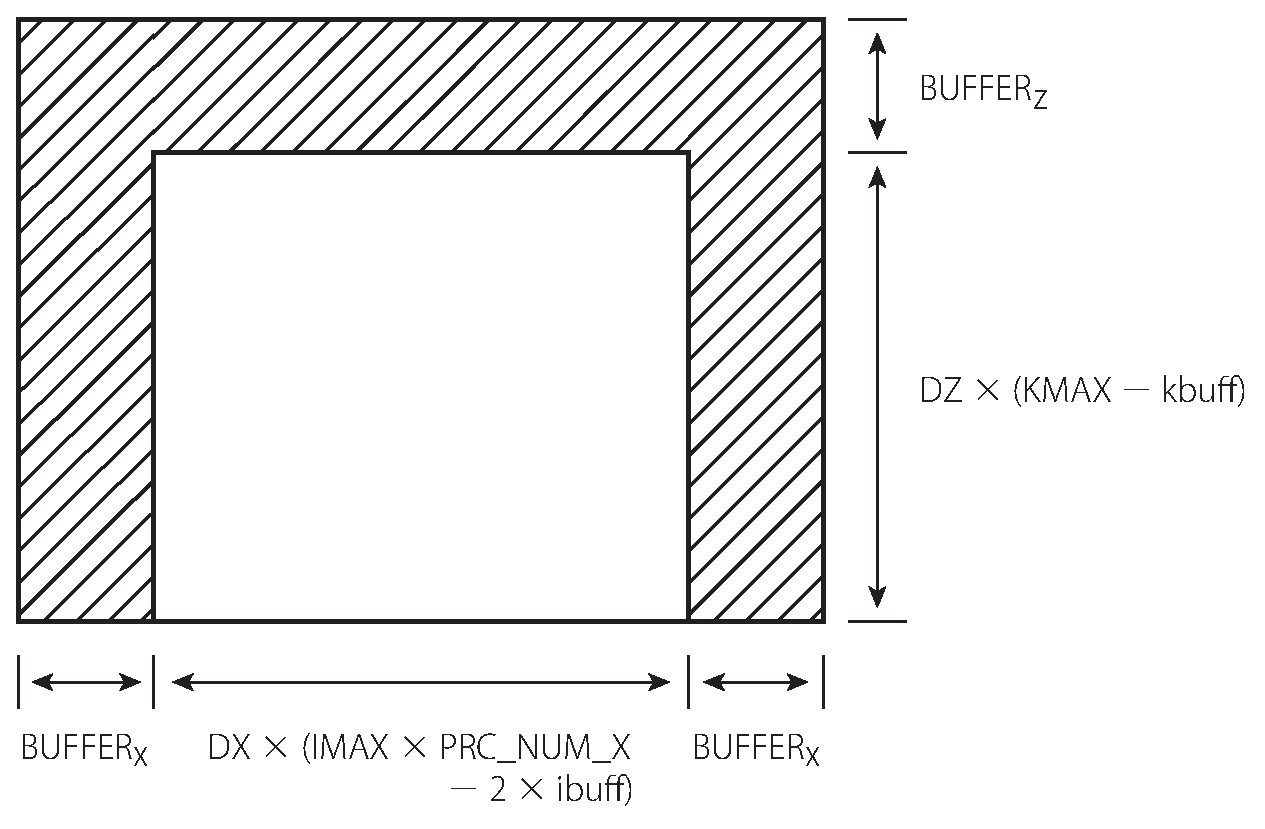
\includegraphics[width=0.8\hsize]{./figure/buffer_xz.eps}\\
  \caption{Location of the buffer region in the entire calculation domain: the shaded area indicates the buffer region. This figure shows the XZ cross-section. It is the same as the YZ cross-section.}
  \label{fig:buff_xz}
\end{center}
\end{figure}

In general, there is no clear criterion for setting the width and locating grids in the buffer region.
This depends on a problem to be solved. In \scalerm, the followings are recommended: the number of grids in the vertical buffer region at the top of the model is greater than 5, whereas that in the lateral boundaries is approximately 20$\sim$40. Depending on the experiment, it may be necessary to increase the number of grids in the buffer region, to increase the buffer region itself by using the appropriate stretch factor, to tune relaxation time, and so on.
The relaxation time is defined as the time
where the difference between the simulated value and the target value becomes $1/e$.
%This relaxation time is given in \nmitem{ATMOS_BOUNDARY_taux, ATMOS_BOUNDARY_tauy, ATMOS_BOUNDARY_tauz}
This relaxation time is given in \nmitem{ATMOS_BOUNDARY_taux, ATMOS_BOUNDARY_tauy}
in \namelist{PARAM_ATMOS_BOUNDARY} in units of seconds.
The default value is ten times as large as \nmitem{TIME_DT}. 
Please refer to section \ref{sec:timeintiv} for \nmitem{TIME_DT}.


%-----------------------------------------------------------------------
\subsubsection{Method for stretching grid intervals in buffer region}
%-----------------------------------------------------------------------

The grid intervals in the buffer region are the same as \nmitem{DX, DY, DZ} in \namelist{PARAM_GRID} by default.
But, it is possible for them to be stretched by setting \nmitem{BUFFFACT} $>$ 1. This specification of \nmitem{BUFFFACT} is applied in all directions if the grid intervals are uniformly specified. When the stretched factor is configured separately in every direction, specify \nmitem{BUFFFACT_X, BUFFFACT_Y, BUFFFACT_Z}. Note that in case of the configuration of vertical levels by giving \nmitem{FZ(:)} (refer to \ref{subsec:gridinterv}), the above stretched settings have no effect along the vertical direction.

The grid interval \verb|BDX| in the buffer region is determined as follows:
\begin{eqnarray}
 \verb|BDX(|n\verb|)| &=& \verb|DX| \times \verb|BUFFFACT|^n, \nonumber
\end{eqnarray}
where $n$ denotes the index of grids in the buffer region, in the order directed from the inner to the outer region in the domain. The grid interval is the same as the inner domain at \nmitem{BUFFFACT=1.0}, whereas it increases from the inner to the outer region by a factor of 1.2 at \nmitem{BUFFFACT=1.2}.  Although any value of \nmitem{BUFFFACT} can be configured, the value from 1.0 to 1.2 is recommended to avoid numerical instability.

Finally, the width of the buffer region $\verb|BUFFER|_{\verb|X|}$ is as follows:
\begin{eqnarray}
  \verb|BUFFER|_{\verb|X|} = \nmitemeq{DX} \times \frac{ \nmitemeq{BUFFFACT}^{\texttt{\detokenize{ibuff}}}-1}{ \nmitemeq{BUFFFACT}-1 }
\end{eqnarray}
Even if the same width of buffer region \nmitem{BUFFER_DX} is specified, the number of grids in the buffer region decreases with increasing \nmitem{BUFFFACT}.
When given by \nmitem{BUFFER_NX}, only the width of buffer region is changed.
